\documentclass[tikz, border=8pt]{standalone}
\usepackage{tikz}
\usepackage{helvet}
\renewcommand{\familydefault}{\sfdefault}
\usetikzlibrary{arrows.meta, calc}

% Okabe-Ito colors
\definecolor{mcpblue}{HTML}{0072B2}
\definecolor{skillorange}{HTML}{D55E00}
\definecolor{toolgreen}{HTML}{009E73}
\definecolor{darkgray}{HTML}{333333}

\begin{document}
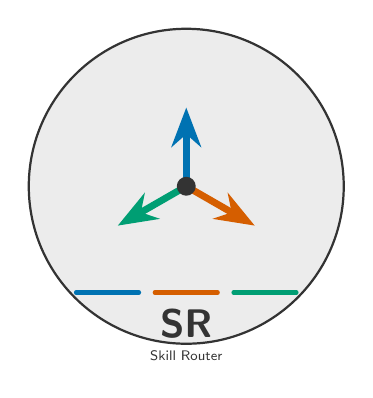
\begin{tikzpicture}[
    >=Stealth,
    line cap=round,
    line join=round
]

% Background circle (subtle)
\fill[lightgray!30] (0,0) circle (2.0cm);
\draw[darkgray, line width=0.8pt] (0,0) circle (2.0cm);

% Compass / router symbol — abstract 4-way arrow
\draw[mcpblue, line width=2.5pt, ->] (0,0) -- (0, 1.0);
\draw[skillorange, line width=2.5pt, ->] (0,0) -- (0.87, -0.5);
\draw[toolgreen, line width=2.5pt, ->] (0,0) -- (-0.87, -0.5);

% Center dot
\fill[darkgray] (0,0) circle (0.12cm);

% Three horizontal lines suggesting layers
\draw[mcpblue, line width=1.5pt] (-1.4, -1.35) -- (-0.6, -1.35);
\draw[skillorange, line width=1.5pt] (-0.4, -1.35) -- (0.4, -1.35);
\draw[toolgreen, line width=1.5pt] (0.6, -1.35) -- (1.4, -1.35);

% Text
\node[font=\bfseries\Large, text=darkgray] at (0, -1.75) {SR};
\node[font=\tiny, text=darkgray] at (0, -2.15) {Skill Router};

\end{tikzpicture}
\end{document}
